%% ---------------------------------------------------------------------------
%% paper/main.tex -- PLB-class letter, plans/07 WP6 (T22-T26, T28).
%%
%% DRAFT v0, 2026-09-16, for the authors' review.
%% Reviewed 2026-09-16 (physics and prose pass, run 19 R-PAPER): the tensor
%% sign of Eq. (1) put into the HJM/HERMES convention the generator carries,
%% the bag normalization of Eq. (4) given its own symbol and its constraint,
%% the seven-|t|-bin fit quoted on the tagging-optics footing it was
%% measured on, the reference tag labelled as such wherever it is quoted.
%%
%% The body carries no run narration and no self-description: it is written as
%% the submitted paper would read.  What follows is for the authors only.
%%
%% SOURCING RULE.  Every line of the body that quotes a number ends with a
%% "% src:" comment naming the report section, plan section or build artifact
%% that number comes from ("R1 sec 5.1" is the Report 1 section of
%% reports/cos2phi_money_plots_report.template.html; "figs/fig2.json" is the
%% file a figure driver wrote).  A displayed equation carries the same comment
%% on the line above it.  tools/checks/paper_numbers.py enforces this, and the
%% same module refuses any form retired in tools/retired_numbers.json.
%%
%% FIGURES AND TABLE 1 ARE GENERATED (T23/T25).  Figures 1-4 are built by
%% paper/fig1_phase_space.py ... fig4_coherent.py, which import the machinery of
%% the producing scripts registered in figs/README.md; their captions and
%% Table 1 are generated from the same arrays, so no numeral in a caption or a
%% table cell is typed into this file.
%%
%% FOOTING.  Single-fill estimator, toy structure functions with a placeholder
%% R, generator level -- the footing Report 1 publishes.  The two-fill
%% estimator (plans/07 SS 7.1) and the nuclear-grid backend (plans/07 WP1
%% addendum) are bounded in Sec. 6 and are author calls, not adopted here.
%%
%% Build: bash build.sh   (see README.md).
%% ---------------------------------------------------------------------------
%% Layout.  Both lines are elsarticle two-column, which is what plans/07 WP6
%% asks for, and the text is identical between them; only the page count is
%% not.  `final,5p,times,twocolumn` is the journal's own layout and is the
%% default because it is the one the length of a letter can be judged in: it
%% sets the four figures and Table 1 beside the text they belong to and runs
%% 7 pages.  `preprint,twocolumn,12pt` -- the scaffold's original line, kept
%% below -- defers every double-column float to the end of the document and
%% runs 16 pages, 4 of them nothing but floats.  Uncomment it to get that.
\documentclass[final,5p,times,twocolumn]{elsarticle}
%\documentclass[preprint,twocolumn,12pt]{elsarticle}

%% hyperref loads `url` itself, so the option has to be passed ahead of it;
%% without it a DOI string in the reference list is one unbreakable box, and
%% xurl lets the remaining ones break anywhere.  Neither reaches the body.
\PassOptionsToPackage{hyphens}{url}

\usepackage[T1]{fontenc}
\usepackage{amsmath}
\usepackage{amssymb}
\usepackage{graphicx}
\usepackage{booktabs}
\usepackage{siunitx}
\usepackage{xurl}
\usepackage[colorlinks=true,allcolors=blue]{hyperref}

%% The reference list prints long DOI strings that cannot be hyphenated;
%% without a little give they overrun the column.  Neither setting changes a
%% line of the body.  The URL glue is kept small: at "plus 2mu" it dominated
%% the stretch of a justified line and letter-spaced every arXiv number.
\emergencystretch=3em
\Urlmuskip=0mu plus 0.1mu\relax

\graphicspath{{figs/}}

%% Figure captions.  Each is written by the driver that builds the figure it
%% belongs to (paper/fig1_phase_space.py ... fig4_coherent.py), from the same
%% arrays that figure plots, so that a number in a caption cannot drift from
%% the panel beside it; Table 1 is generated whole by paper/table1.py from the
%% drivers' own output.  All five come out of one `bash build.sh`, which is
%% what plans/07 SS 7.8 asks for.  Do not edit the generated files.
% paper/figs/fig1_caption.tex -- GENERATED by the fig1 driver.
% Do not edit: rebuild with paper/build.sh.
\newcommand{\figonecaption}{%
The $(x, Q^{2})$ phase space of the measurement at $e(10\,\mathrm{GeV}) \times {}^{6}\mathrm{Li}\,(99.5\,\mathrm{GeV/u})$ for a one-year programme (10\,fb$^{-1}$ per nucleon). Colour: expected inclusive DIS events per bin of the $40 \times 30$ log--log analysis grid, drawn where at least one event is expected, after the scattered-electron cuts $|\eta| \le 3.5$, $E' \ge 0.5$\,GeV, $0.01 \le y \le 0.95$ and $W^{2} \ge 10$\,GeV$^{2}$ (dashed: the $y$ and $W^{2}$ boundaries). Vermillion: the four $\cos 2\phi'$ super-bins of Table~\ref{tab:projections}; thin dark lines: the merged $x$ bins of the $\Delta$ extraction along the sweet-spot $Q^{2}$ slices. Green: the coherent channel over the same grid, as contours of the tagged rate at $10^{4}$ and $10^{5}$ recoils per bin per year for a scenario coherent fraction $f_{0} = 0.04$ dying at $x_{\rm coh} = 0.01$ and a near-beam $p_{T} > 0.20$\,GeV tag of acceptance $13.5\%$, with the box of its highest-yield super-bin. One year gives $5.2\times10^{9}$ inclusive events, $1.2\times10^{8}$ coherent and $1.7\times10^{7}$ tagged.%
}

% paper/figs/fig2_caption.tex -- GENERATED by the fig2 driver.
% Do not edit: rebuild with paper/build.sh.
\newcommand{\figtwocaption}{%
Inclusive $\cos 2\phi'$ projections at $e(10\,\mathrm{GeV}) \times {}^{6}\mathrm{Li}\,(99.5\,\mathrm{GeV/u})$ with $P_{zz} = 0.60$. (a), (b): the $\phi'$ distribution of the two super-bins that span the accepted phase space, $x = 0.0282$, $Q^{2} = 1.14$\,GeV$^2$ and $x = 0.141$, $Q^{2} = 14.3$\,GeV$^2$, as one-year pseudo-data (10\,fb$^{-1}$ per nucleon) with statistical errors, against the injected modulation (solid) and the binned fit (dashed); the fits return $\hat A = (7.31 \pm 0.17)\times10^{-3}$ and $(8.88 \pm 0.45)\times10^{-3}$ per unit $P_{zz}$. (c): the amplitude extracted in 10 merged $x$ bins along the $Q^{2} = 1.14$\,GeV$^{2}$ slice, with independent one-year (open) and ten-year (filled, 100\,fb$^{-1}$ per nucleon) pseudo-measurements, against the moment-constrained $\Delta$ that was injected, the no-$F_{1}$ variant and a flat $\Delta/F_{1} = 10^{-3}$ reference. All four super-bins, including the two not drawn here, are tabulated in Table~\ref{tab:projections}. Statistical errors only; the $\Delta$ model carries the $^{6}$Li per-nucleon dilution $1/3$.%
}

% paper/figs/fig3_caption.tex -- GENERATED by the fig3 driver.
% Do not edit: rebuild with paper/build.sh.
\newcommand{\figthreecaption}{%
The double-helicity-flip structure function extracted from the amplitudes of Fig.~\ref{fig:inclusive}, at $e(10\,\mathrm{GeV}) \times {}^{6}\mathrm{Li}\,(99.5\,\mathrm{GeV/u})$ with $P_{zz} = 0.60$: $x\Delta(x, Q^{2})$ per nucleon in the $Q^{2} = 1.14$\,GeV$^{2}$ (a) and $Q^{2} = 14.3$\,GeV$^{2}$ (b) slices, with independent one-year (open, 10\,fb$^{-1}$ per nucleon) and ten-year (filled, 100\,fb$^{-1}$ per nucleon) pseudo-measurements against the injected moment-constrained $\Delta$ and the no-$F_{1}$ variant. Each point is the fitted amplitude of a pair of merged $x$ bins converted to a point value by the model bin-centring factor $K = \Delta_{\rm model}(x_{c}, Q^{2}_{c})/A_{\rm model}$, so that $\delta\Delta = \delta\hat A\,|K|$. The best bin of each slice reaches $\Delta = -0.135 \pm 0.003$ at $x = 0.02$ and $-0.0047 \pm 0.0004$ at $x = 0.316$ in one year, 2.5\% and 9.5\% relative. The two curves are separated bin by bin at low $Q^{2}$ and cross at large $x$ in the high-$Q^{2}$ slice, which is what makes the $x$ dependence, rather than the size of the amplitude, the discriminating measurement. Statistical errors only; the third sweet-spot slice, $Q^{2} = 3.13$\,GeV$^{2}$, is measured with the same draw and is not drawn here.%
}

% paper/figs/fig4_caption.tex -- GENERATED by the fig4 driver.
% Do not edit: rebuild with paper/build.sh.
\newcommand{\figfourcaption}{%
The coherent channel $e\,^{6}\mathrm{Li} \to e' X\,^{6}\mathrm{Li}(\mathrm{g.s.})$ at $e(10\,\mathrm{GeV}) \times {}^{6}\mathrm{Li}\,(99.5\,\mathrm{GeV/u})$ with $P_{zz} = 0.60$. (a) The deformation coefficient $a_{2}(|t|)$: the digitized polarized-deuteron anchor per magnetic substate, against the $^{6}$Li ensemble band obtained by scaling it with $\varepsilon_{B0} \in -(0.04\text{--}0.13)$ (central value $-0.08$), whose sign is opposite to the deuteron's because $Q(^{6}\mathrm{Li}) < 0$. The shaded strip is the analysis window $0.017$--$0.25$\,GeV$^{2}$ and the dotted line the form-factor zero at $|t| = 0.31$\,GeV$^{2}$, above which the linear model does not hold. Inset: the tagged fraction of coherent recoils against the near-beam envelope. The assumption it rests on is the cutout geometry: the three blue curves assume a rectangular cutout $2.5$ times as wide as it is high, an illustrative aspect ratio rather than the measured one, at $B = 40$, $50$ and $60$\,GeV$^{-2}$ (dotted, solid, dashed), the grey curve is the circular $e^{-B p_{T}^{2}}$ the rate model itself uses at $B = 50$\,GeV$^{-2}$, and the marker is the $p_{T} > 0.20$\,GeV working point at which that model gives $13.5\%$. No $^{6}$Li optics delivering this envelope is published, which is why the acceptance is shown as a curve and not as a point. (b) The $\phi'$ distribution of the tagged sample in the highest-yield super-bin, $x \in [1.26, 2.51]\times10^{-3}$, $Q^{2} \in [1.00, 1.66]$\,GeV$^{2}$, holding $1.75\times10^{6}$ recoils in one year (10\,fb$^{-1}$ per nucleon) for a coherent fraction $f_{0} = 0.04$: pseudo-data with statistical errors against the deformation-anchored $\langle a_{2}\rangle_{\rm tag} = 0.036$ at $P_{zz} = 0.60$ (solid) and the binned fit (dashed), with the flat gluon-transversity scenario (grey, $0.006$) for scale. The fit returns $\hat A = (58.9 \pm 1.8)\times10^{-3}$ per unit $P_{zz}$ against $0.060$ injected, i.e.\ $5\sigma$ floors of $9.0\times10^{-3}$ in one year and $2.9\times10^{-3}$ in ten (Table~\ref{tab:projections}). Statistical errors only; backgrounds, purity and tensor radiative corrections are not included.%
}


%% BIBLIOGRAPHY SWITCH.  refs.bib holds exactly the 35 works this letter
%% cites, in exact correspondence with the \cite commands below; the 40
%% further records that cover the reference lists of Report 1 and of
%% docs/note_cos2phi_coherent_6Li.md, and that this text does not stand on,
%% are the reserve in refs_reserve.bib.  \draftbibtrue adds that reserve and
%% emits \nocite{*}, so that `bash build.sh` is also a check that every
%% record of both files parses and prints; the letter itself is built with
%% \draftbibfalse and compiles refs.bib alone.
\newif\ifdraftbib
\draftbibfalse

\journal{Physics Letters B}

\begin{document}

\begin{frontmatter}

%% Title candidate (a) of plans/07 SS 7.5, which that section recommends (D5).
%% Candidates (b) and (c) are recorded there; D5 is an author call.
\title{Nuclear gluonometry with a tensor-polarized $^{6}$Li beam at the
       Electron-Ion Collider}

%% Authorship is D3 of plans/07 SS 7.7: lead C. Peng, second author J. Zhou.
%% The co-authors that section lists as candidates to invite are NOT added here.
\author[anl]{C.~Peng}
\author[anl]{J.~Zhou}
\address[anl]{Physics Division, Argonne National Laboratory,
              Lemont, Illinois 60439, USA}

\begin{abstract}
The double-helicity-flip structure function $\Delta(x,Q^{2})$ of a spin-1
target is generated at leading twist by gluons alone and has never been
measured.
We project its measurement at the Electron-Ion Collider with a transversely
tensor-polarized $^{6}$Li beam.
In inclusive scattering, one year at $10$\,fb$^{-1}$ per nucleon resolves the % src: R1 sec 3.1
$\cos 2\phi$ amplitude at $21$--$43\sigma$ in four $(x,Q^{2})$ bins and returns % src: R1 sec 5.1
$x\Delta$ to $2$--$9\%$, so that its $x$ dependence discriminates between % src: R1 sec 5.1
moment-constrained interpretations.
In coherent diffraction with the $^{6}$Li intact, the same modulation separates
a nuclear-shape term, predicted to flip sign relative to the polarized
deuteron, from exotic glue; the anomalously small quadrupole moment of
$^{6}$Li makes that a null test.
We state what beam, spin direction and far-forward system each channel
requires.
\end{abstract}

\begin{keyword}
Electron-Ion Collider \sep tensor polarization \sep gluon transversity \sep
$^{6}$Li \sep coherent diffraction
\end{keyword}

\end{frontmatter}

%% ---------------------------------------------------------------------------
%% Sec. 1 -- Introduction.  Budget 600 words (plans/07 SS 7.5).
%% ---------------------------------------------------------------------------
\section{Introduction}
\label{sec:intro}

A spin-1 target can absorb two units of photon helicity in the forward Compton
amplitude. The structure function that measures this, $\Delta(x,Q^{2})$,
receives no leading-twist contribution from quarks or from bound spin-$\tfrac{1}{2}$
nucleons, so in a nucleus it is direct evidence for glue that is not inherited
from the individual nucleons --- exotic glue, in the language of nuclear
gluonometry~\cite{Jaffe:1989xy,Hoodbhoy:1988am}. At order $\alpha_{s}$ it is
generated by the gluon transversity distribution $\delta G$, an interference of
gluon helicity states that exists only for $J \ge 1$.

$\Delta$ has never been measured. The only prior experimental document is a
letter of intent for a $^{14}$N target, which carries no sensitivity
projection~\cite{Maxwell:2018gci}. The absolute normalizations available are
moment estimates, and they disagree by an order of magnitude: a bag-model
calculation for the spin-$\tfrac{3}{2}$ $\Delta^{++}$ gives
$\int x\Delta\,\mathrm{d}x = -0.012\,\alpha_{s}$~\cite{Sather:1990bq}; % src: R1 sec 2
lattice QCD gives a non-zero gluon transversity in the $\phi$ meson at
$m_{\pi} = 450$\,MeV~\cite{Detmold:2016gpy} and, for the deuteron at % src: R1 sec 2
$m_{\pi} \approx 806$\,MeV, a moment $-0.010(3)$ whose % src: R1 sec 2
transversity-to-momentum ratio is roughly ten times below the
$\phi$'s~\cite{Winter:2017bfs}; and percent-level asymmetries
appear only in proton--deuteron Drell--Yan under the maximal-transversity
assumption its authors call optimistic~\cite{Kumano:2019igu}. Nothing exists
for $^{6}$Li or for any $A > 2$ nucleus beyond a $\Delta\Delta$-isobar estimate
for the deuteron~\cite{Nzar:1992ax}, so the literature brackets the nuclear
$\Delta$ in both directions: suppressed, as in the lattice deuteron, or
enhanced by binding in analogy with the EMC effect.

Three properties make $^{6}$Li the practical target. It is a polarized deuteron
bound to an inert $\alpha$ particle, by $1.47$\,MeV against % src: R0 sec 2.2
$\alpha + d$ breakup~\cite{Tilley:2002vg}, so its tensor observables can be set
against the free deuteron's. It is among the easiest ions to store polarized:
its gyromagnetic anomaly, $G \approx -0.18$, is as small as the deuteron's, so it % src: R0 sec 2.3
crosses $81$ depolarizing resonances on the way to top energy against $63$ for % src: R0 sec 2.3
the deuteron and $2457$ for $^{3}$He, and the stable spin direction in the arcs % src: R0 sec 2.3
is vertical, which makes a transverse alignment axis the native
configuration~\cite{EPIOSScientificConsortium:2025dfc}. And its quadrupole
moment is anomalously small, $Q = -0.0806(6)$\,fm$^{2}$ against % src: R1 sec 6.3
$+0.286$\,fm$^{2}$ for the free deuteron~\cite{Stone:2016bmk}, the result of a % src: R0 sec 2.2
cancellation between the deuteron's own moment and the $D$-wave part of the
$\alpha$--$d$ relative motion that theory reproduces only in
magnitude~\cite{Wiringa:1998hr}; that near-sphericity is what turns the
coherent channel into a null test.

This letter presents the first numerical projection of a $\Delta$ measurement
for any target, and the first treatment of the coherent channel on a polarized
nucleus beyond the deuteron. To our knowledge neither exists in the literature:
the letter of intent above is the only prior experimental document and states
no reach, and the polarized-nucleus coherent-diffraction programme opened by the
colour-glass calculation of Ref.~\cite{Mantysaari:2024xmy} has not been extended
past $A = 2$, its authors' subsequent work on light nuclei being
unpolarized~\cite{Mantysaari:2026dps}.

%% ---------------------------------------------------------------------------
%% Sec. 2 -- The observable.  Budget 450 words.
%% ---------------------------------------------------------------------------
\section{The observable}
\label{sec:observable}

For unpolarized electrons on a spin-1 target whose alignment axis makes an
angle $\theta_{m}$ with the beam, the inclusive cross section per spin
projection $m$ is~\cite{Jaffe:1989xy,Hoodbhoy:1988am}
% src: R1 sec 2
\begin{multline}\label{eq:master}
\frac{\mathrm{d}\sigma^{(m)}}{\mathrm{d}x\,\mathrm{d}y\,\mathrm{d}\phi}
 = \frac{2y\alpha^{2}}{Q^{2}}\bigg[F_{1}\\
 - \tfrac{2}{3}a_{m}b_{1}
   + \frac{1-y}{xy^{2}}\Big(F_{2} - \tfrac{2}{3}a_{m}b_{2}\Big)\\
 - \frac{1-y}{y^{2}}\,c_{m}\sin^{2}\theta_{m}\,\Delta\cos 2\phi\bigg],
\end{multline}
% src: R1 sec 2
with $a_{m} = \tfrac{1}{4}c_{m}(3\cos^{2}\theta_{m}-1)$,
$c_{m} = 3|\lambda_{m}| - 2 \rightarrow (1,-2,1)$ and $\phi$ the azimuth of the
lepton plane about the virtual photon, measured from the transverse projection
of the alignment axis. Averaged over a fill, $c_{m}$ becomes the tensor
polarization $P_{zz} = p_{+} + p_{-} - 2p_{0}$. The tensor terms carry the sign
convention of HERMES and of Cosyn \emph{et al.}~\cite{HERMES:2005pon,Cosyn:2024drt},
$A_{zz} = -\tfrac{2}{3}\,b_{1}/F_{1}$ for an alignment axis along the % src: R1 sec 2
photon. At leading order $\Delta$ is
the photon--gluon convolution of the gluon transversity distribution,
% src: R1 sec 2
\begin{equation}\label{eq:deltag}
\begin{split}
\Delta(x,Q^{2}) = -\frac{\alpha_{s}(Q^{2})}{2\pi}&\Big(\sum_{q}e_{q}^{2}\Big)\\
 &\times\, x^{2}\!\int_{x}^{1}\!\frac{\mathrm{d}y}{y^{3}}\,\delta G(y,Q^{2}),
\end{split}
\end{equation}
so the explicit $\alpha_{s}$ is the Wilson coefficient of the box and the
$\mathcal{O}(\alpha_{s})$ suppression relative to $F_{1}$ is
model-independent, while the size of $\delta G$ is not. For a transverse
alignment axis, $\theta_{m} = 90^{\circ}$, the measured amplitude per unit % src: R1 sec 2
$P_{zz}$ and its inversion are
% src: R1 sec 2
\begin{equation}\label{eq:amp}
\begin{gathered}
A^{\cos 2\phi} = -\frac{1-y}{y^{2}}\frac{\Delta}{D_{\phi}},\qquad
\hat{\Delta} = -\hat{A}\,\frac{y^{2}D_{\phi}}{1-y},\\
D_{\phi} = F_{1} + \frac{1-y}{xy^{2}}F_{2}.
\end{gathered}
\end{equation}

Three properties of Eq.~(\ref{eq:amp}) shape the analysis. With
$F_{2} = 2x(1+R)F_{1}$ the inversion becomes
$\Delta/F_{1} = -\hat{A}\,[2(1+R) + y^{2}/(1-y)]$, in which the $y^{2}$ term
is negligible at the $y \lesssim 0.03$ of the sensitive region, so that % src: R1 sec 2
$R = \sigma_{L}/\sigma_{T}$ is the only structure-function input that reaches
$\Delta/F_{1}$. The amplitude is
exactly linear in $\Delta$, which is what allows the response to be applied as
a linear operator rather than as a model-dependent bin-centring factor
(Sec.~\ref{sec:inclusive}). And target-mass corrections are small: at the
analysis bins $\gamma^{2} = 4M^{2}x^{2}/Q^{2} \le 0.0057$, where the exact % src: R1 sec 2
longitudinal kernel collapses to a multiplicative $(1+\gamma^{2})$ worth
$\le 0.6\%$, and no $\Delta$ reported here is built from a longitudinal % src: R1 sec 2
asymmetry.

One finite-$\gamma$ effect is physical rather than kinematic: because
an axis transverse to the beam is not transverse to the photon, the
tensor-polarized $b_{1}$--$b_{4}$ terms feed the $\cos 2\phi$ amplitude at
$\mathcal{O}(\gamma^{2})$. Evaluated with the exact spin-1
kernel~\cite{Cosyn:2024drt} this leakage is an effective $\Delta$ of
$(0.14$--$0.16)\,\gamma^{2}b_{1}$, worth at most $0.033\%$ of the amplitude at % src: R1 sec 2
the bins used here, and of the sign that opposes rather than fakes a negative
$\Delta$. Since $99.96\%$ of it is carried by $b_{2} = 2xb_{1}$ at leading % src: R1 sec 2
twist, it is the same combination that the $\phi$-independent constant of the
spin-state ratio measures, and is subtractable in situ from the same fills;
what that leaves is the unmeasured $b_{3}$, $b_{4}$ band, $0.6$ of the leakage. % src: R1 sec 2

%% ---------------------------------------------------------------------------
%% Sec. 3 -- Simulation framework.  Budget 500 words.  Asset: Fig. 1.
%% ---------------------------------------------------------------------------
\section{Simulation framework}
\label{sec:framework}

EIC ions are $\gamma$-matched to the proton rather than rigidity-scaled,
because the two rings share a revolution period, so the $^{6}$Li menu is
$40.8$\,GeV/u and $99.5$--$137.5$\,GeV/u, the top value being the rigidity cap % src: R1 sec 3.1
$275\,\mathrm{GeV}\times Z/A$~\cite{AbdulKhalek:2021gbh,EPIOSScientificConsortium:2025dfc}. % src: R1 sec 3.1
Projections are made at the mid configuration,
$e(10\,\mathrm{GeV}) \times {}^{6}\mathrm{Li}(99.5\,\mathrm{GeV/u})$, % src: R1 sec 3.1
$\sqrt{s_{NN}} = 63$\,GeV. The in-ring tensor polarization is a placeholder % src: R1 sec 3.1
$P_{zz} = 0.6$ --- the source targets $P_{zz} \ge 0.8$ and transport to the % src: R1 sec 3.1
ring is an open accelerator question --- the alignment axis is the vertical,
and the electrons are unpolarized. Luminosity is quoted per nucleon:
$10$\,fb$^{-1}$/u for one EIC year, the Yellow Report's $30$ weeks at % src: R1 sec 3.1
$10^{33}$\,cm$^{-2}$s$^{-1}$ with $60\%$ % src: R1 sec 3.1
efficiency~\cite{AbdulKhalek:2021gbh}, and $100$\,fb$^{-1}$/u for a ten-year % src: R1 sec 3.1
programme. No lithium luminosity has been published and the yields scale
linearly with whatever the machine delivers.

No public generator produces polarized $e+A$ events for $A>1$. The generator
used here implements the missing component --- the spin-density matrix
$\otimes$ structure-function master formula of Eq.~(\ref{eq:master}) with
spin-correlated sampling --- and takes its hadronic final state from a
PYTHIA\,8 production; it is validated against the analytic asymmetry formulas
and by pseudo-experiments, including unbiased $\cos 2\phi$ recovery under
azimuthal acceptance holes~\cite{Peng:Report2}. Structure functions are toy
parameterizations with PDF-grid backends behind one interface, so rates hold to
a factor $\approx 1.5$ and asymmetry shapes are scenarios by construction; % src: R1 sec 3.2
$R$ is a placeholder of the right magnitude, $0.14$--$0.18$ at the analysis % src: R1 sec 3.2
bins, and Sec.~\ref{sec:systematics} carries the shift to the measured
fit~\cite{E143:1998nvx} as a correction to apply.

Rates use per-nucleon luminosity and the scattered-electron cuts
$|\eta| \le 3.5$, $E' \ge 0.5$\,GeV, $0.01 \le y \le 0.95$ and % src: R1 sec 3.4
$W^{2} \ge 10$\,GeV$^{2}$, which accept $5.2\times10^{9}$ events in one year % src: R1 sec 3.4
(Fig.~\ref{fig:phasespace}). Four $(x,Q^{2})$ super-bins are selected by
statistical significance within $Q^{2}$ bands, each merging $3\times3$ cells of % src: R1 sec 3.4
a $40\times30$ logarithmic grid ($3\times2$ for the two at % src: R1 sec 3.4
$Q^{2} = 1.14$\,GeV$^{2}$, clipped at the grid's $Q^{2} = 1$\,GeV$^{2}$ edge); % src: R1 sec 3.4
they sit at $y = 0.010$, $0.025$, $0.011$ and % src: R1 sec 3.4
$0.025$, because the amplitude grows as $(1-y)/y^{2}$ and the sensitivity lives % src: R1 sec 3.4
at the lowest $y$ the detector can reconstruct.

The figures use a single spin state and a binned least-squares fit of
$N(\phi') = C(1 + A\cos 2\phi')$, with $\phi'$ the covariant
azimuth~\cite{Bacchetta:2006tn} and
$\delta A = \sqrt{2/N}/P_{zz}$ validated by pseudo-experiments. The
measurement itself cannot use a single state, because that fit also measures
the detector's own $\cos 2\phi'$ acceptance harmonic divided by $P_{zz}$: a
$3\%$ harmonic aligned with the alignment axis fakes an amplitude of $0.05$, % src: R1 sec 3.3
five to eleven times the signal. The estimator is therefore the spin-state
ratio of $m = \pm1$-rich and $m = 0$-rich bunches, which cancels any acceptance
common to both states and gives
$\delta \hat{A} = 2\sqrt{2/N}/(P_{+}-P_{0})$, $0.67$ times the single-state % src: R1 sec 3.3
error if the $m = 0$-rich fill reaches $|P_{zz}| = 1.2$ at equal % src: R1 sec 3.3
purity~\cite{Peng:Report2}. Its cancellation is not free: a $10^{-3}$ % src: R1 sec 3.3
difference of the harmonic between the two fills fakes $5.6\times10^{-4}$, % src: R1 sec 3.3
six to thirteen per cent of the projected amplitudes, so bunch-by-bunch % src: R1 sec 3.3
alternation is a requirement of the measurement rather than a refinement.

%% Drawn at one column (3.375 in) by paper/fig1_phase_space.py.  The width
%% key is a no-op that guards against a future column-width change; the PDF
%% is already exactly one column wide, and scaling it would move every
%% declared 8 pt off 8 pt.
\begin{figure}[t]
  \centering
  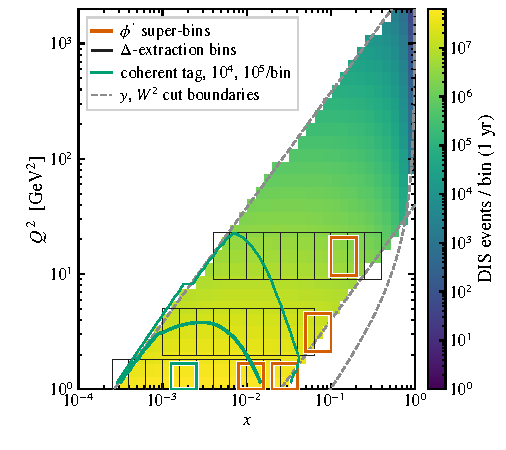
\includegraphics[width=\linewidth]{fig1.pdf}
  \caption{\figonecaption}
  \label{fig:phasespace}
\end{figure}

%% ---------------------------------------------------------------------------
%% Sec. 4 -- Inclusive projections.  Budget 700 words.  Figs. 2-3, Table 1.
%% ---------------------------------------------------------------------------
\section{Inclusive projections}
\label{sec:inclusive}

The size of $\Delta$ is unknown to within an order of magnitude, so the
projections carry a model normalized to the bag moment and applied to the
per-nucleon $\Delta$ of $^{6}$Li,
% src: R1 sec 4
\begin{equation}\label{eq:model}
\Delta_{\mathrm{A}}(x,Q^{2}) = \frac{\mathcal{N}}{3}\alpha_{s}(Q^{2})F_{1}(x,Q^{2})
   \frac{x^{a}(1-x)^{b}}{N_{\mathrm{peak}}},
\end{equation}
with $(a,b) = (0.7,3)$, $N_{\mathrm{peak}}$ the peak value of $x^{a}(1-x)^{b}$, % src: R1 sec 4
and $\mathcal{N} = -0.292$ fixed by % src: R1 sec 4
$\int_{0}^{1} x\Delta\,\mathrm{d}x = -0.012\,\alpha_{s}$ for the undiluted % src: R1 sec 4
ansatz at the rate-weighted $\langle Q^{2}\rangle = 4.47$\,GeV$^{2}$ of the % src: R1 sec 4
accepted phase space. The factor $1/3$ restricts % src: R1 sec 4
the exotic glue to the polarized deuteron-like pair while the whole-nucleus
$P_{zz}$ remains a separate factor; it is a counting fraction and not a
polarization~\cite{Peng:Report0}. A second model imposes the same moment
without the $F_{1}$ factor and gives amplitudes a factor $3$--$56$ lower at the % src: R1 sec 4
four bins, and the spread between the two is the dominant ansatz systematic.
Porting a single-hadron bag moment to a per-nucleon nuclear structure function
has no precedent, so normalization and $x$ dependence are both scenario
choices.

Figure~\ref{fig:inclusive} shows the $\phi'$ pseudo-data in two of the four
super-bins and the amplitude extracted along the $Q^{2} = 1.14$\,GeV$^{2}$ % src: figs/fig2.json
slice; Table~\ref{tab:projections} gives all four. The injected amplitudes are
$7.4$, $4.4$, $9.5$ and $9.5 \times 10^{-3}$ per unit $P_{zz}$ against one-year % src: R1 sec 5.1
statistical errors of $1.7$, $1.4$, $2.7$ and $4.5 \times 10^{-4}$ --- $43$, % src: R1 sec 5.1
$31$, $35$ and $21\sigma$ --- and the fitted values agree with the injected % src: R1 sec 5.1
ones within $1.5$ standard errors. Under the moment constraint the measurement % src: R1 sec 5.1
is not a null test: the spread between the two models is resolved by the $x$
dependence of the amplitude, and a flat amplitude of $3\times10^{-3}$ per unit % src: R1 sec 5.1
$P_{zz}$ would remain a $3$--$11\sigma$ effect per bin even at % src: R1 sec 5.1
$P_{zz} = 0.3$. At ten-year precision the statistical errors sit below the % src: R1 sec 5.1
polarimetry scale systematic, so that measurement is systematics-limited.

%% Drawn at the full text width (7.0 in) by paper/fig2_inclusive.py, hence
%% figure* rather than figure.
\begin{figure*}[t]
  \centering
  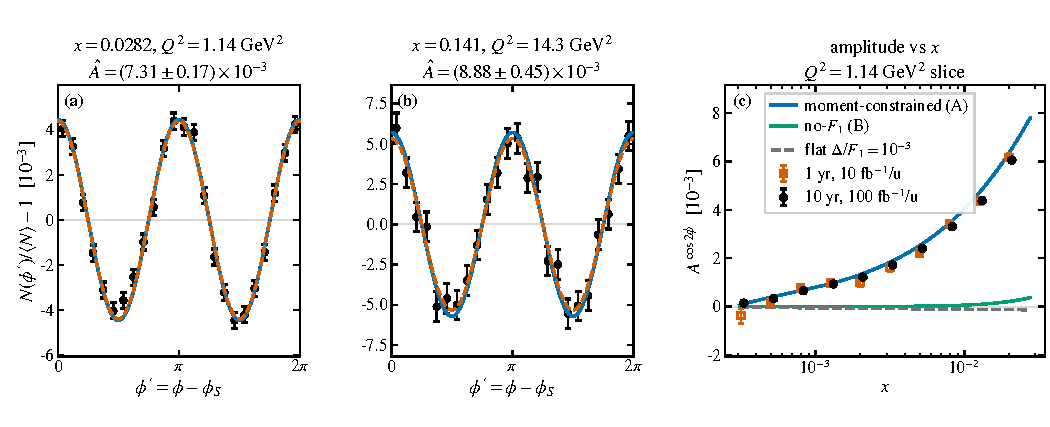
\includegraphics[width=\linewidth]{fig2.pdf}
  \caption{\figtwocaption}
  \label{fig:inclusive}
\end{figure*}

Figure~\ref{fig:extraction} unfolds the same pseudo-measurements to the
structure function itself. The best bins reach
$\Delta = -0.135 \pm 0.003$ at $(x,Q^{2}) = (0.02, 1.14)$, % src: R1 sec 5.1
$-0.070 \pm 0.002$ at $(0.05, 3.13)$ and $-0.0047 \pm 0.0004$ at % src: R1 sec 5.1
$(0.32, 14.3)$ in one year, i.e.\ $2$--$9\%$ relative, and three times better % src: R1 sec 5.1
in ten. The two curves are separated bin by bin at low $Q^{2}$ and cross at
large $x$ in the high-$Q^{2}$ slice, which is why the $x$ dependence rather
than the size of the amplitude is the discriminating measurement.
Figure~\ref{fig:extraction} converts amplitude to $\Delta$ with the model's own
bin-centring factor, which as an analysis would be circular; because
the amplitude is exactly linear in $\Delta$, the response can instead be applied
as a linear operator and a $\Delta(x)$ shape fitted through it per $Q^{2}$
slice, which reduces the model dependence of the correction over the plotted
bins from as much as $29\%$ to $\le 6\%$~\cite{Peng:Report2}. % src: R1 sec 5.3

%% Drawn at one column by paper/fig3_extraction.py.
\begin{figure}[t]
  \centering
  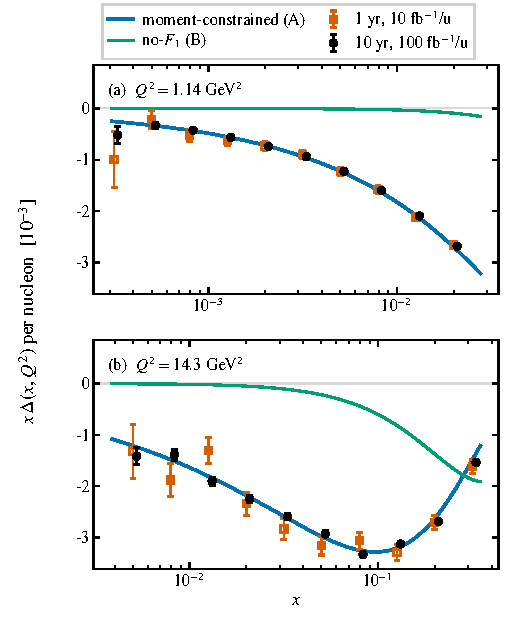
\includegraphics[width=\linewidth]{fig3.pdf}
  \caption{\figthreecaption}
  \label{fig:extraction}
\end{figure}

%% Table 1 is generated whole -- float, caption and cells -- by
%% paper/table1.py, out of figs/fig2.json and figs/fig4.json, which the
%% figure drivers wrote.  It is labelled tab:projections.
%% paper/table1.tex -- GENERATED by paper/table1.py; do not edit.
%% Every number is read out of paper/figs/fig2.json and fig4.json,
%% which the figure drivers wrote from their own pseudo-experiments.
\begin{table*}[t]
  \centering
  \caption{Projected statistical precision for the double-helicity-flip observable at $e(10\,\mathrm{GeV}) \times {}^{6}\mathrm{Li}\,(99.5\,\mathrm{GeV/u})$ with $P_{zz} = 0.60$, in one-year and ten-year EIC programmes (10 and 100\,fb$^{-1}$ per nucleon). $A$ is the injected $\cos 2\phi'$ amplitude per unit $P_{zz}$ and $\delta\hat A$ the statistical error on the fitted amplitude on the same footing. The four inclusive rows are the analysis super-bins of Fig.~\ref{fig:inclusive}, each of $3\times3$ grid cells ($3\times2$ for the two clipped at the grid\'s $Q^2 = 1$\,GeV$^2$ edge), with $\Delta$ the moment-constrained ansatz normalized to $\int x\Delta\,\mathrm{d}x = -0.012\,\alpha_s$ at $\langle Q^2\rangle = 4.47$\,GeV$^2$ and carrying the $^{6}$Li per-nucleon dilution $1/3$. The coherent row is the tagged-count-maximal super-bin of the intact-recoil channel behind a near-beam $p_T > 0.20$\,GeV tag, which keeps $13.5\%$ of the coherent recoils for $f_0 = 0.04$ and $B = 50$\,GeV$^{-2}$, a reference envelope that no published IP6 optics delivers (Sec.~\ref{sec:coherent}); its amplitude is the deformation-anchored $\langle a_2\rangle_{\mathrm{tag}} = 0.060$ per unit $P_{zz}$, i.e.\ $0.036$ at $P_{zz} = 0.60$ over a band $0.018$--$0.059$, and its $5\sigma$ detection floors are $9.01\times10^{-3}$ (one year) and $2.85\times10^{-3}$ (ten years) per unit $P_{zz}$ (Fig.~\ref{fig:coherent}). Errors are statistical only; backgrounds, purity, polarimetry and tensor radiative corrections are not included. Every entry is produced by the drivers that build Figs.~\ref{fig:phasespace}--\ref{fig:coherent}, from the same seeds as those figures.}
  \label{tab:projections}
  \begin{tabular}{@{}l r r r r r@{}}
    \toprule
    bin $(x,\ Q^{2}\,[\mathrm{GeV}^{2}])$ & $N$ (1\,yr) & $A$ $[10^{-3}]$ & $\delta\hat A$ (1\,yr) $[10^{-3}]$ & $\delta\hat A$ (10\,yr) $[10^{-3}]$ & $A/\delta\hat A$ \\
    \midrule
    \multicolumn{6}{@{}l}{\emph{inclusive} $\cos2\phi'$, scattered electron only} \\
    $(0.0282,\ 1.14)$ & $1.90\times10^{8}$ & $7.42$ & $0.173$ & $0.0547$ & $43$ \\
    $(0.0112,\ 1.14)$ & $2.81\times10^{8}$ & $4.35$ & $0.142$ & $0.0450$ & $31$ \\
    $(0.0708,\ 3.13)$ & $7.52\times10^{7}$ & $9.49$ & $0.275$ & $0.0869$ & $35$ \\
    $(0.141,\ 14.3)$ & $2.85\times10^{7}$ & $9.52$ & $0.446$ & $0.141$ & $21$ \\
    \midrule
    \multicolumn{6}{@{}l}{\emph{coherent} $e\,^{6}\mathrm{Li}\to e'X\,^{6}\mathrm{Li}$(g.s.), intact recoil tagged} \\
    $(1.26\text{--}2.51)\times10^{-3},\ 1.00\text{--}1.66$ & $1.75\times10^{6}$ & $60.0$ & $1.80$ & $0.570$ & $33$ \\
    \bottomrule
  \end{tabular}
\end{table*}


Two of the four super-bins sit at $y \approx 0.01$, where the electron method % src: R1 sec 5.2
alone does not reconstruct the bin, so $x$ must come from a hadronic-method
$y$. Passing every event through calorimeter and tracking smearing, an
$\eta$-dependent electron identification, the analysis cuts on reconstructed
quantities and the spin-state ratio with an acceptance harmonic and a
relative-luminosity offset switched on, the fit closes on the response-folded
truth and the errors are $0.60$--$0.72$ of the single-state truth-level % src: R1 sec 5.2
values~\cite{Peng:Report2}. With the hadronic scale calibrated from simulation
in bins of the reconstructed $(x,Q^{2})$, as an analysis would, the bin
purities are $0.56$--$0.75$ and the reconstructed-bin amplitude is within % src: R1 sec 5.2
$7\%$ of the true-bin value; the real final state costs purity rather than % src: R1 sec 5.2
statistics, since only $70$--$85\%$ of the hadronic $E-p_{z}$ sum survives the % src: R1 sec 5.2
acceptance and the threshold~\cite{ATHENA:2022hxb}. Unfolded, the best
reconstructed bins reach $\delta\Delta = 2.4\times10^{-3}$ at % src: R1 sec 5.2
$Q^{2} = 1.14$\,GeV$^{2}$ and $1.2\times10^{-3}$ at $3.13$\,GeV$^{2}$ in one % src: R1 sec 5.2
year. What controls those purities is the calorimeter noise floor on the
hadronic sum, a regime no published ePIC study covers, which makes it the
central detector question for this measurement.

%% ---------------------------------------------------------------------------
%% Sec. 5 -- The coherent channel.  Budget 700 words.  Asset: Fig. 4.
%% ---------------------------------------------------------------------------
\section{The coherent channel}
\label{sec:coherent}

In coherent diffraction, $e\,^{6}\mathrm{Li} \to e'X\,^{6}\mathrm{Li}$(g.s.),
the nucleus stays in its ground state and the modulation of the tagged yield
mixes two mechanisms that separate by their $t$ dependence. No diffractive
prediction exists for a light nucleus, so the coherent share is a scenario
band,
% src: R1 sec 6.2
\begin{equation}\label{eq:fcoh}
\begin{gathered}
f_{\mathrm{coh}}(x) = \frac{f_{0}}{1 + (x/x_{\mathrm{coh}})^{2}},\\
f_{0} = 0.04\ [0.02\text{--}0.08],
\end{gathered}
\end{equation}
with $x_{\mathrm{coh}} = 0.01$ from diffractive practice and a slope % src: R1 sec 6.2
$B = 50$\,GeV$^{-2}$ $[40$--$60]$ from $B = \langle r^{2}\rangle/3$ with the % src: R1 sec 6.2
matter radius~\cite{Sick:2015spa}, valid below the form-factor minimum at
$|t| \approx 0.31$\,GeV$^{2}$~\cite{Suelzle:1967zz}. The band sits below both % src: R1 sec 6.2
anchors available, HERA $ep$ diffraction at $10$--$15\%$ of % src: R1 sec 6.2
DIS~\cite{H1:2012pbl} and heavy-nucleus saturation estimates at
$20$--$25\%$~\cite{Kowalski:2008sa}, a loosely bound $A = 6$ nucleus taking the % src: R1 sec 6.2
smaller share. One year then produces $1.2\times10^{8}$ coherent events, of % src: R1 sec 6.2
which a reference tag with a $0.20$\,GeV near-beam envelope, one that no % src: R1 sec 6.2
published IP6 optics delivers (below), keeps $1.7\times10^{7}$; the % src: R1 sec 6.2
highest-yield super-bin of
Table~\ref{tab:projections} holds $1.75\times10^{6}$ and gives $5\sigma$ floors % src: R1 sec 6.2
of $0.9\%$ and $0.3\%$ per unit $P_{zz}$ in one and ten years on that footing. % src: R1 sec 6.2

The deformation term is scaled from the polarized-deuteron colour-glass
calculation of Ref.~\cite{Mantysaari:2024xmy}, the only published calculation
of polarization-dependent azimuthal coefficients in coherent diffraction on any
polarized nucleus. Its coefficients grow linearly in $|t|$ with
$a_{2}(m{=}0) \approx -2a_{2}(m{=}\pm1)$, the wave-function-symmetry relation, % src: R1 sec 6.3
from the $D$-wave modulating the diffractive slope; for a fill of populations % src: R1 sec 6.3
$p_{m}$ the ensemble coefficient is proportional to $P_{zz}$,
% src: R1 sec 6.3
\begin{equation}\label{eq:a2}
\begin{gathered}
a_{2}(t;P_{zz}) = -\frac{P_{zz}}{4}\,\varepsilon_{B0}\,B\,|t|,\\
\langle a_{2}\rangle_{\mathrm{tag}}
  = a_{2}\!\left(p_{T,\mathrm{cut}}^{2}+1/B\right).
\end{gathered}
\end{equation}
The relative slope modulation $\varepsilon_{B0}$ is scaled from the deuteron's
$0.21$ by two indicators that disagree: the relative quadrupole deformation of % src: R1 sec 6.3
$^{6}$Li is about one fifth of the deuteron's and opposite in sign, while the
$\alpha$--$d$ asymptotic $D/S$ ratio is disputed --- a transfer measurement
gives $\eta = +0.0003(9)$~\cite{Veal:1999yk}, consistent with zero, and the % src: R1 sec 6.3
\emph{ab initio} no-core shell model with continuum gives
$-0.027$~\cite{Hupin:2014iqa}, the deuteron's own value in % src: R1 sec 6.3
magnitude. We adopt $\varepsilon_{B0} \in -(0.04$--$0.13)$ with default % src: R1 sec 6.3
$-0.08$, leaving near-zero deformation open. That puts % src: R1 sec 6.3
$\langle a_{2}\rangle_{\mathrm{tag}}$ at $0.036$ at $P_{zz} = 0.6$, a band % src: R1 sec 6.3
$0.018$--$0.059$ on that footing and $0.060$ per unit $P_{zz}$, which is the % src: R1 sec 6.3
footing of Table~\ref{tab:projections} (Fig.~\ref{fig:coherent}). The anchor's own
convention makes the observable modulation twice this coefficient, so the
coherent reaches quoted here are conservative by a factor two. The band's width
is genuine theoretical uncertainty: even exact few-body calculations miss the
$^{6}$Li quadrupole cancellation by a factor
$\approx 3$~\cite{Wiringa:1998hr}, and the gluonic deformation need not share % src: R1 sec 6.3
the cancellation of the charge sector.

%% Drawn at the full text width by paper/fig4_coherent.py.
\begin{figure*}[t]
  \centering
  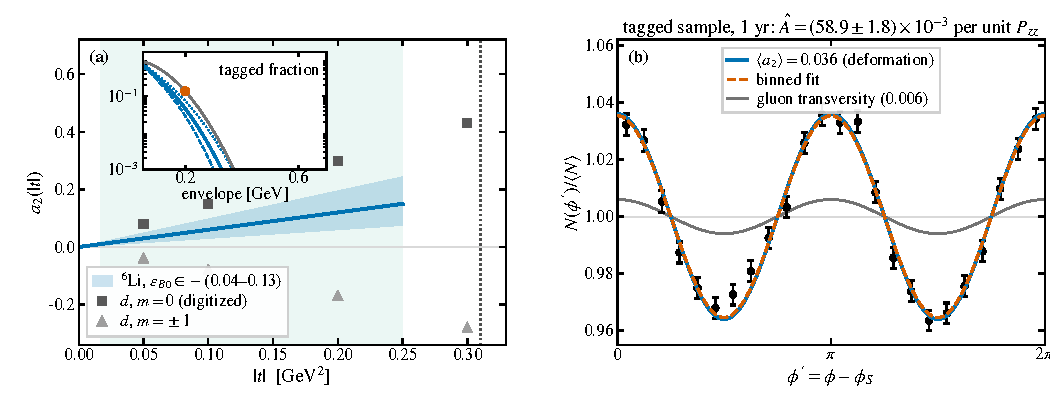
\includegraphics[width=\linewidth]{fig4.pdf}
  \caption{\figfourcaption}
  \label{fig:coherent}
\end{figure*}

The second term, gluon transversity proper, is flat in $t$ and persists at
small $x$, where it connects to the elliptic-gluon
programme~\cite{Hatta:2016dxp}; it is separately bounded at
$3\times10^{-3}$--$10^{-2}$ at $P_{zz} = 1$ from the lattice inputs of % src: R1 sec 6.3
Sec.~\ref{sec:intro}. The two therefore separate in a two-component fit
$a_{2}(t) = c_{\mathrm{def}}|t| + a_{g}$, and it is $^{6}$Li that makes the
separation clean: a deformation-driven modulation is bounded by the quadrupole
moment, $Q(^{6}\mathrm{Li}) \approx Q(^{7}\mathrm{Li})/50$, so a sizable % src: R1 sec 6.3
flat-in-$t$ $\cos 2\phi$ on $^{6}$Li cannot be a shape effect --- the null test
unavailable to the deuteron --- while the shape term itself is predicted to
flip sign relative to the deuteron because $Q(^{6}\mathrm{Li}) < 0$. Incoherent
breakup is blind to the magnetic substate in this mechanism: it dilutes the
modulation but cannot mimic it. Tensor modulations of comparable size are
established at these $|t|$: HERMES measured $A_{zz}(d) \approx -1\%$ at % src: R1 sec 6.3
$x \approx 0.01$~\cite{HERMES:2005pon}, attributed to coherent double % src: R1 sec 6.3
scattering~\cite{Nikolaev:1996jy}.

Detecting the intact recoil is the difficulty, and it is where the channel
turns into a requirement. The recoil keeps the beam's rigidity --- $A/Z = 2$
exactly, and the diffractive momentum loss changes it by less than
$1\%$ --- and emerges within a milliradian of the beam, so of the far-forward % src: R1 sec 6.1
system at IP6 only the Roman Pots can see it~\cite{Jentsch:2021qdp}, and only
where it clears both the beam envelope and the pots' own aperture. With an
exponential $t$ distribution both constraints act on the angle at the
interaction point,
% src: R1 sec 6.1
\begin{equation}\label{eq:tag}
\begin{gathered}
\varepsilon_{\mathrm{tag}} = e^{-Bp_{T,\mathrm{cut}}^{2}},\qquad
p_{T,\mathrm{cut}} = \theta_{\mathrm{cut}}Ap_{u},\\
\theta_{\mathrm{cut}} = \max(10\sigma_{\theta},\theta_{\mathrm{ap}}),
\end{gathered}
\end{equation}
an exponential in the square of the beam divergence times the beam momentum.
Evaluated with the published divergences and an aperture measured by tracking
an intact $^{6}$Li through the current ePIC geometry, the tagged fraction at
the three configurations is at most $10^{-5}$ under either constraint alone % src: R1 sec 6.1
and below $10^{-9}$ under both: with any published % src: R1 sec 6.1
optics the channel does not exist at IP6~\cite{Peng:Report3,Peng:Report4}. It
exists under either of two conditions. A dedicated tagging optics --- the
horizontal $\beta^{*}$ raised by $46$, $164$ and $89$ with the vertical plane % src: R1 sec 6.1
untouched, the pots following the envelope --- recovers a $25$--$37\%$ tag at % src: R1 sec 6.1
$1/6.8$ to $1/12.8$ of the luminosity, $2.4$ to $6.1 \times 10^{6}$ tagged % src: R1 sec 6.1
events per year, and asks the pots to approach a factor $6.9$, $7.9$ and $4.5$ % src: R1 sec 6.1
closer than the silicon edge the present geometry holds. On the counting floor
of its best super-bin alone that is an $8$--$11\sigma$ measurement of the shape % src: R1 sec 6.1
term per year and a $5\sigma$ one of a $1\%$ flat term in three to six % src: R1 sec 6.1
years; the fit of the whole tagged sample at the same optics, in seven $|t|$
bins spanning $0.017$--$0.25$\,GeV$^{2}$, measures the flat term to % src: R1 sec 6.3
$\delta a_{g} = 0.0007$--$0.0012$ per unit $P_{zz}$ per % src: R1 sec 6.1
year~\cite{Peng:Report2}, and that fit, rather than any single super-bin, is
the measurement. Alternatively the secondary focus of a second interaction
region reaches
$p_{T} \approx 0$, with published intact-recoil efficiencies of $47\%$ for the % src: R1 sec 6.1
deuteron and $17.8\%$ for $^{7}$Li~\cite{Chang:2025pgi}; no $^{6}$Li case is % src: R1 sec 6.1
published, and our interpolation of $\approx 20\%$ would be worth $4$ to $10$ % src: R1 sec 6.1
times the IP6 optimum at equal luminosity. One degeneracy survives either
choice: a pot hit measures $A/Z$, and an intact $^{6}$Li, an $\alpha$ and a $d$
at the same velocity share trajectory and timing. The $\alpha + d$ channel,
open at $1.47$\,MeV~\cite{Tilley:2002vg}, is accordingly the background that % src: R1 sec 6.4
decides the purity; it is handled by the two-component $|t|$ fit, benchmarked
at $80$--$99\%$ incoherent rejection in $e+$Pb~\cite{Chang:2021jnu}, and by the % src: R1 sec 6.4
partner deuteron, which at the tagging optics lands on a pot in $84\%$ of the % src: R1 sec 6.1
events in which an $\alpha$ fakes the tag~\cite{Peng:Report4}.

%% ---------------------------------------------------------------------------
%% Sec. 6 -- Systematics and assumptions.  Budget 450 words (T28).
%% ---------------------------------------------------------------------------
\section{Assumptions}
\label{sec:systematics}

Every number above is statistical and rests on inputs that are stated rather
than fitted. The structure functions are toy parameterizations with a
placeholder $R$; the grid backends behind the same interface hold the rates to
a factor $\approx 1.5$, and replacing the placeholder by the measured % src: R1 sec 3.2
fit~\cite{E143:1998nvx} moves $\Delta/F_{1}$ by $+18$, $+18$, $+8$ and $-4\%$ % src: R1 sec 3.2
at the four bins --- a correction to apply, and the systematic on every
$\Delta$ quoted here until it is. A nuclear PDF set can be used in place of the
toy $F_{2}^{A}$, and doing so lowers the accepted rate by a factor $0.77$ and % src: plans/07 sec 7.4
the tagged coherent yield by $0.70$, leaving the four significances at % src: plans/07 sec 7.4
$18$--$28\sigma$; but the set has no support below $Q^{2} = 1.69$\,GeV$^{2}$, % src: plans/07 sec 7.4
where $8.7\%$ of the accepted cells and $36.3\%$ of the accepted rate lie, and % src: plans/07 sec 7.4
two of the four bins and the whole coherent super-bin sit there, so no claim is
made on that footing below that scale.

The $1/3$ of Eq.~(\ref{eq:model}) is a counting fraction of the polarized pair
among six nucleons. Whether $\Delta$, a rank-2 quantity, should instead carry
the rank-2 $\alpha$--$d$ transfer of $0.92$ as $b_{1}$ does --- an $8\%$ % src: R1 sec 4
reduction --- is left open, and no projection assumes it. The tensor
polarimetry scale is taken as $\delta P_{zz}/P_{zz} \le 5\%$, a $1{:}1$ % src: R1 sec 7
normalization on $\hat{\Delta}$ that still requires dedicated
development~\cite{EPIOSScientificConsortium:2025dfc}.
Radiative corrections for tensor observables have not been calculated, and no
unpolarized study stands in for them. The unpolarized part is bounded rather
than assumed: collinear initial-state radiation cannot fake a $\cos 2\phi'$,
cancels in the spin-state ratio, and moves only the $Q^{2}$ label of the bin,
which biases $\hat{\Delta}$ by $+0.5$ to $+1.2\%$ at the four bins and by at % src: R1 sec 7
most $2.9\%$ with the low-$Q^{2}$ feed-in opened up, against the $5\%$ gate set % src: R1 sec 7
for this projection~\cite{Peng:Report2}. Detector nuisances were measured with
common random numbers rather than argued: a $\pm1\%$ electron energy scale % src: R1 sec 7
moves $\hat{\Delta}$ by $0.3$--$1.0\%$, a hadronic-resolution mismatch by % src: R1 sec 7
$0.5$--$1.4\%$ and a $1\%$ residual hadronic-scale error by % src: R1 sec 7
$0.1$--$0.6\%$. The $\mathcal{O}(\gamma^{2})$ tensor leakage of % src: R1 sec 7
Sec.~\ref{sec:observable} is carried as a systematic rather than applied as a
correction. In interpretation, a $\Delta\Delta$-isobar admixture can mimic
$\Delta$ at leading twist~\cite{Nzar:1992ax} and conventional double scattering
generates the low-$x$ $b_{1}$~\cite{Nikolaev:1996jy}; the $Q^{2}$ lever arm and
the $^{6}$Li/$d$ comparison discriminate against both.

Three assumptions carry the coherent numbers and none of them is a
measurement: that a near-beam tag exists at all, in the sense of
Sec.~\ref{sec:coherent}; the coherent fraction, for which no light-nucleus
prediction exists; and $\varepsilon_{B0}$, whose two indicators disagree by a
factor three. The analysis also assumes the impulse approximation with no
final-state interactions, and a linear $a_{2}(t)$ only below
$|t| = 0.2$\,GeV$^{2}$, the form-factor zero above being excluded rather than % src: R1 sec 6.2
modelled. Finally, every projection here takes the whole year in its own spin
configuration and far-forward optics, so the inclusive and coherent reaches are
alternatives rather than a sum; each scales as the inverse square root of the
share the run plan gives it.

%% ---------------------------------------------------------------------------
%% Sec. 7 -- Summary and outlook.  Budget 250 words.
%% ---------------------------------------------------------------------------
\section{Summary and outlook}
\label{sec:summary}

A transversely tensor-polarized $^{6}$Li beam at the EIC measures
$\Delta(x,Q^{2})$ in inclusive deep inelastic scattering at $21$--$43\sigma$ % src: R1 sec 8
per $(x,Q^{2})$ bin in one year under the moment-constrained scenario, and at
$3$--$11\sigma$ per bin for a flat amplitude of $3\times10^{-3}$ per unit % src: R1 sec 8
$P_{zz}$ even at $P_{zz} = 0.3$, discriminating between interpretations of the % src: R1 sec 8
bag moment by the $x$ dependence and returning $x\Delta(x,Q^{2})$ to
$2$--$9\%$ in the best bins. The result survives reconstruction, at the price % src: R1 sec 8
of bin purities that the calorimeter noise floor controls.

The measurement makes three demands on the machine that are specific and
answerable: tensor polarization delivered as alternating $m = \pm1$-rich and
$m = 0$-rich bunches, transverse at the interaction point; a $\cos 2\phi'$
acceptance harmonic stable to $10^{-4}$ between the spin states, and a pot % src: R1 sec 8
envelope stable to $10^{-3}$ ($10^{-4}$ in the three $|t|$ bins below % src: R1 sec 8
$0.05$\,GeV$^{2}$), or the bunch-by-bunch alternation that makes a % src: R1 sec 8
relative-luminosity error a constant; and a tensor polarimetry scale at the
few-per-cent level.

The coherent channel carries the same physics with a null test the deuteron
cannot offer, and it is a requirement rather than a projection: the intact
$^{6}$Li cannot be tagged at IP6 with any published optics, at any energy, and
what recovers it is a dedicated tagging optics or the secondary focus of a
second interaction region. The highest-leverage inputs from outside are, on the
machine side, a light-ion optics with $\beta^{*}$ chosen for tagging and a
charge-identification study of the pot readout; on the theory side, a
polarized-nucleus colour-glass calculation with an $\alpha$--$d$ cluster
density, a lattice $\Delta$ moment for a light nucleus, and radiative
corrections for tensor observables.

\section*{Acknowledgments}
We thank the EIC polarized-ion-source and far-forward communities for
discussions. This work was supported by the U.S.\ Department of Energy, Office
of Science, Office of Nuclear Physics.
Writing assisted by Claude (Anthropic).

\bibliographystyle{elsarticle-num}
\ifdraftbib\nocite{*}\bibliography{refs,refs_reserve}\else\bibliography{refs}\fi

\end{document}
